\documentclass{article}
\usepackage[utf8]{inputenc}

\usepackage{graphicx}
\usepackage{float}
\usepackage{enumerate}

\title{Project Imacs: System Requirements Specifications}
\author{Group 16:\\ Kelvin Lin\\ Jiahong Dong\\ Liam Casola\\ Varun Hooda\\ Mikolaj Hrycko\\ Danish Khan\\ Prince Sandu\\ Baltej Toor }
\date{November 2\textsuperscript{nd} 2018}

\begin{document}

\maketitle
\newpage
\tableofcontents
\newpage
\section{Introduction}
This section outlines the purpose and scope of Project Imacs, along with definitions, acronyms, and abbreviations used within this document. Its purpose is to set the context for the contents and organization of the software requirement document.

\subsection{Purpose}
This document's purpose is to outline the engineering and business decisions made in designing Project Imacs. This document will be used to maintain a record of the project's scope, constraints, assumptions, dependencies, functional requirements, non-functional requirements, and any other design decisions made over the life of this project.

The target audience for this document are the stakeholders of this projects as well as any future software architects, designers, developers, and engineers.

\subsection{Scope}
This project will produce the following software products:

\begin{itemize}
    \item A desktop client application.
    \item A custom-made file system mapping a non-linear file structure to a linear one.
\end{itemize}

The aforementioned product will perform the following:

\begin{itemize}
    \item Provide users with a graphical interface to organize files in a semantically consistent manner.
    \item Provide users with a graphical interface to create and edit files.
    \item Provide a means of persistent storage and retrieval of files.
\end{itemize}

The aforementioned product will not perform the following:

\begin{itemize}
    \item Alter files outside the software ecosystem.
    \item Persist files outside the user's local machine.
    \item Infer relationships between files.
    \item Automatically populate files with content.
\end{itemize}

\subsection{Definitions, Acronyms, and Abbreviations}
\subsubsection{File}
A file is a collection of data stored on the computer that can be intepreted into human-usable information by a computer.

\subsubsection{Group of Files}
A group of files is a user-defined non-empty set of files that are related to each other.

\subsubsection{Jump}
A jump is an operation that allows users to navigate the view between two related groups of files.

\subsubsection{Label}
A label is a unique user-defined textual description assigned to a group of files to provide semantics for that group of files.

\subsubsection{Relation}
A relation is a link between two different groups of files.

\subsubsection{Tag}
A tag is a user-defined textual description assigned to provide context to a file.

\subsection{References}
This section is void.

\subsection{Overview}
The rest of this document contains detailed descriptions of the project's design decisions: assumptions, functionality, functional requirements, and non-functional requirements.

The other sections are organized into logical subsections. Section 2 outlines the overall product description with its various subsections. Section 3 will list the requirements. The functional requirements are organized by business events and viewpoints. Non-functional requirements are organized into various subcategories.

\section{Overall Description}
\subsection{Product Perspective}
Our system is an independent cross-platform desktop note-taking system with the ability to manage files. It allows the user to take notes in a non-linear file traversal system along a hierarchical file system. Users will be able to view and modify their files as well as the relation between files. Besides for the desktop operating system, such as but not limited to Windows and MacOS, the note-taking and file management system will not rely on any external software product. Nevertheless, in order to capture input from the user, the system requires either a keyboard, mouse, or touchpad. Users may choose to use a sketchpad or a digital pen instead of the aforementioned input systems and output devices. Some of the functionality in the system may require the use of external APIs; however, APIs will only act as add-on modules, and the core system that abstracts away hierarchical file management in the note-taking process will not be affected by the use of APIs.

Similar systems to Project Imacs include Microsoft OneNote and Emacs. These solutions allow users to take and save notes; however, they fail to address the following problems:

\begin{itemize}
    \item They do not allow the user to link physical files on their drive without duplicating the file or its contents resulting in lots of redundant information.
    \item They do not allow for a distributed file handling format, resulting in large files that may be slow to load and corruption to the file may result in a lot of data loss.
    \item The user can manually recreate a non-linear file system by creating separate folders; however, this will not allow them to visualize the relationship between the files.
\end{itemize}

Project Imacs will enable the user to group correlated notes in groups and non-hierarchically save them to the local machine.

\subsection{Product Functions}
In addition to the general note-taking functions that can be found in similar products, Project Imacs allows users to tag their notes, create relationship between correlated notes based on tags, and put these notes into groups. Users will be able to attache desired files to their notes. Users will also be able to save their notes in a non-hierarchical fashion on their local machines.

\subsection{User Characteristics}
Our note-taking system is intended for the general computer user with the desire to take notes and organize them in a non-linear manner. Potential users could be high school students, university students, working age adults, and mature adults.

\subsection{Constraints}
The system shall be constrained only by the user's operating system, and the physical computer hardware configurations.

\subsection{Assumptions and Dependencies}
It shall be assumed that the user does not violate any of the operating system's constraints. It shall also be assumed that the user is able and willing to use the appropriate hardware peripherals required to operate the system.
It shall be assumed that the user agrees to the terms and conditions of any licensing requirements specified by the APIs used in our application.

\section{Context Diagram}
The following context diagram illustrates the boundary of the Project Imacs system. The data element represent all utilized file system content and metadata. The Graphical User Interface component of Project Imacs provides the interface for the graphical manipulation of the data.

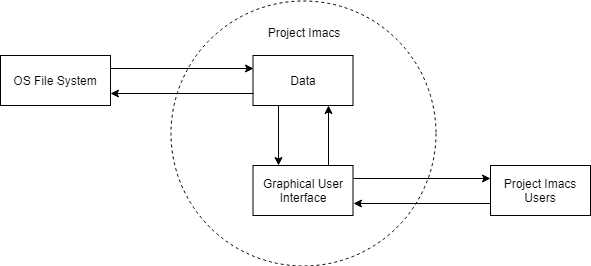
\includegraphics[scale=0.5]{context_diagram.png}

\section{Functional Decomposition Diagram}
The following is a functional decomposition diagram details top-level functional hierarchy of Project Imacs.

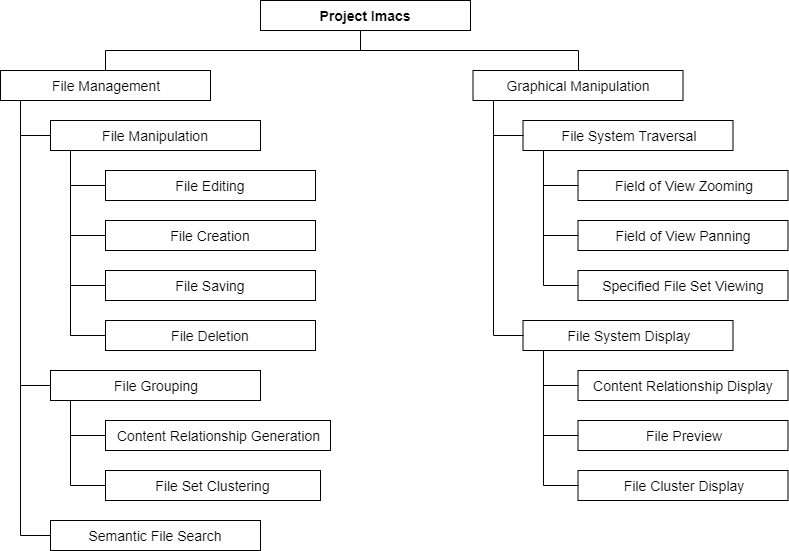
\includegraphics[scale=0.5]{functional_decomposition_diagram.png}

\section{Functional Requirements}
\subsection{Data Requirements}
\begin{enumerate}[DR1]
    \item The system shall allow the creation of files.

	Rationale: The creation of files is needed in order to allow the user to create notes.
	\item The system shall allow the addition of text, pen-input, or images to files.

	Rationale: The addition of text, pen-input, and images is neededed in order for the user to add content to their notes. Text, pen-input, and images were chosen as the required methods of input because it most closely relates to traditional note-taking using pen and paper. Relating Project Imacs to a familliar task will lower the cognitive effort required of the user to learn how to use the software.
    \item The system shall allow the editing of files.

	Rationale: The editing of files is needed to allow the user to correct mistakes they made while taking notes.

	\item The system shall allow the deletion of content from files.

	Rationale: The deletion of content from files is needed to allow users to remove incorrect, unwanted, or redundant information from their notes.
    \item The system shall allow the saving of files.

	Rationale: The saving of files is needed so that users will not have to re-enter their notes everytime they use the software.
    \item The system shall allow the retrieval of saved files.

	Rationale: The user needs to be able to continue from a saved file or to read information from the saved file so that the information that the user previously entered is not lost.
    \item The system shall allow for the incorporation external files into the software ecosystem.

	Rationale: Some users may have used other note-taking/mindmapping software before Project Imacs, and this requirement will facilitate their transition to Project Imacs resulting in a more intuitive user experience.
    \item The system shall allow files to be assigned tags.

	Rationale: Having a tag on files will allow users to provide context and descriptions for a file, and it will also facilitate the semantic search function defined in DR14, and the visualization requirement defined in UIR3.
    \item The system shall allow files to be grouped together.

	Rationale: Allowing files to be grouped together will allow the system to better visualize the relationship between files in requirement UIR2. It will also facilitate the semantic search function defined in requirement DR14.
    \item The system shall allow a label to be assigned to a group.

	Rationale: Allowing a label to be assigned to a group will enable the computer to visualize the label defined in UIR4, and it will aid in the semantic search function defined in requirement DR14.
    \item The system shall allow relationships to be specified between groups of files.

	Rationale: Allowing relationships to be specified between groups of files will allow the user to draw conclusions about how different notes relate to each other.
    \item The system shall allow modification of the relationships between groups of files.

	Rationale: Allowing the modification of relationships between groups of files is needed because the relationship between different group of files may change, and notes that were related in the past may not be related in the future.
    \item The system shall allow jumping between related groups of files.

	Rationale: Quick navigation between related groups of files is needed in order to facilitate an intuitive user experience.
    \item The system shall allow searching for files semantically.

	Rationale: Current note-taking and mind-mapping software does not allow users to search for content semantically; instead, they only allow users to search in-line text using exact word search or regular expression matching. Allowing users to search semantically will provide a better user experience that more naturally mimics human thought.

    \item The system shall allow the deletion of files.
	
	Rationale: The deletion of files is needed because the user will want to delete any notes that are no longer needed.
\end{enumerate}

\subsection{User Interface Requirements}
\begin{enumerate}[U{I}R1]
    \item The system shall display the files stored within its ecosystem.
    \item The system shall visualize the relationship between groups of files.
	\item The system shall display the tags associated with a file when the file is highlighted.
	\item The system shall display the label associated with a group of files when the group of files is presented on an output device.
    \item The system shall show an interface for manipulating human-readable files.
    \item The system shall allow navigation between relationships between groups of files.
    \item The system shall allow users to change the notes visible on their screen.
    \item The system shall render images and plaintext files in a human usable format.
\end{enumerate}

\section{Non-Functional Requirements}
\subsection{Look and Feel Requirements}
\subsubsection{Appearance Requirements}
\begin{enumerate}[{A}PR1]
    \item The application shall use appropriate font styling given the type and location of the text.
    \item The application shall not have clashing colours that would make readability challenging for the user.
    \item The application shall visually resemble other business and note-taking applications.
    \item The application shall prohibit users from interacting with the interactive elements that lead to invalid operations.
\end{enumerate}

\subsubsection{Style Requirements}
\begin{enumerate}[STR1]
    \item The application shall have a style similar to other applications used in business and professional environments.
    \item The visual style, colour palette, and fonts shall remain consistent throughout the application.
\end{enumerate}

\subsection{Usability and Humanity Requirements}
\subsubsection{Ease of Use Requirements}
\begin{enumerate}[EUR1]
    \item The application shall make the important features stand out.
    \item The application shall make the important features easily accessible.
\end{enumerate}

\subsubsection{Learning Requirements}
\begin{enumerate}[LER1]
    \item The product shall not require more than 2 hours of training before the user can access more than 75\% of the operations specified in the functional requirements.
\end{enumerate}

\subsubsection{Understandability and Politeness Requirements}
\begin{enumerate}[UPR1]
    \item The application shall have intuitive icons and appropriate names to describe the function of its interactive elements.
\end{enumerate}

\subsubsection{Accessibility Requirements}
\begin{enumerate}[{A}CR1]
    \item Text and graphic components shall be clearly distinguishable on the application interface.
    \item The application shall use a font size large enough to allow users to read the text in a brightly lit indoor room.
    \item The application shall be usable by colour blind users.
\end{enumerate}

\subsection{Performance Requirements}
\subsubsection{Speed and Latency Requirements}
\begin{enumerate}[SLR1]
    \item The system shall respond in near real-time except in the cases of file searches and file operations.
    \item The system shall perform search queries in less than 1 second.
    \item The system shall open files and be ready for I/O operations in less than 3 seconds.
\end{enumerate}

\subsubsection{Reliability and Availability Requirements}
\begin{enumerate}[R{A}R1]
    \item The system shall have a 99\% uptime.
    \item The system shall always make all data stored within its ecosystem available to the user through the application and through the user's operating system's default file management system.
\end{enumerate}

\subsubsection{Robustness or Fault-Tolerance Requirements}
\begin{enumerate}[RFR1]
    \item The system will keep data integrity upon spontaneous shutdown.
    \item The system will automatically create backups of data.
\end{enumerate}

\subsubsection{Capacity Requirements}
\begin{enumerate}[CR1]
    \item The system must allow individual file sizes of up to 4GB.
    \item The system must allow total capacity file sizes of at least 128GB.
\end{enumerate}

\subsubsection{Scalability or Extensiblity Requirements}
\begin{enumerate}[SER1]
    \item The system shall be forwards compatible with new file formats.
    \item The system shall be open for addition of new features.
    \item The system shall make its data available in a human-readable, non-proprietary format.
\end{enumerate}

\subsubsection{Longevity Requirements}
\begin{enumerate}[LOR1]
    \item The system shall use current software engineering standards and protocols.
\end{enumerate}

\subsection{Operational and Environmental Requirements}
\subsubsection{Expected Physical Environment Requirements}
\begin{enumerate}[EPE1]
    \item The application shall be used in calm environmental conditions.
\end{enumerate}

\subsubsection{Requirements for Interfacing with Adjacent Systems}
\begin{enumerate}[R{I}{A}1]
    \item The application shall interface with Windows, MacOS, and Linux platforms.
    \item The application shall interface with the files provided by the user.
\end{enumerate}

\subsubsection{Productization Requirements}
\begin{enumerate}[PRO1]
    \item The product shall be distributed as an executable file corresponding to the interfaced platform.
    \item The product shall be offered to users free of charge.
\end{enumerate}

\subsubsection{Release Requirements}
\begin{enumerate}[RR1]
    \item New releases of the product shall be produced in conjunction with stakeholder feedback.
\end{enumerate}

\subsection{Maintainability and Support Requirements}
\subsubsection{Maintenance Requirements}
\begin{enumerate}[MR1]
    \item The software shall not be in maintenance and inaccessible to the user for more than 2 hours each day.
    \item The software shall be maintained at night in North America to affect the least amount of North American users.
\end{enumerate}

\subsubsection{Supportability Requirements}
\begin{enumerate}[SUR1]
    \item The software shall provide access to a help manual.
    \item A tutorial on the application's functionality shall be presented the first time the software is launched.
\end{enumerate}

\subsection{Security Requirements}
\subsubsection{Access Requirements}
\begin{enumerate}[{A}CR1]
    \item The system shall store associated files in a user-accessible location.
\end{enumerate}

\subsubsection{Integrity Requirements}
\begin{enumerate}[{I}NT1]
    \item The system shall not introduce security vulnerabilities to the underlying OS file system structures.
    \item The system shall not create, corrupt, modify, or delete files not managed by the system.
\end{enumerate}

\subsubsection{Privacy Requirements}
\begin{enumerate}[PR{I}1]
    \item The system shall not transmit or share the user's file contents and information.
    \item The system shall explicitly prompt the user to agree to any use of the user's data deviating from the core file management and manipulation functionality.
\end{enumerate}

\section{User Profiles and Personas}
\subsection{User Profiles}
WRITE SOMETHING HERE

\subsection{Personas}
A persona is a hypothetical individual that represents the typical user for Project Imacs. Based on independent research and speaking with people who currently use note taking software, we summarized some common personas for Project Imacs.

\subsubsection{Janet, Student}
Janet is a 20 year old commerce student who is trying to understand how contribution margins effect a company's performance. She has notes on contribution margins; however, contribution margins affect many areas of businesses such as R\&D, marketing, operations, and finance. She wants to be able to relate contribution to each department's performance so that she can get a better sense of how the business performs overall.

\subsubsection{Timothy, Researcher}
Timothy is a 40 year old researcher who classifies organisms for a living. He has notes for every organism he observes; however, he would like to be able to find organisms with similar attributes and group them together. Currently, he has a large database of animals, and he requires the help of an information technology student in order to effectively search and find the database. He would like to be able to visualize the different organisms he documented independently.

\end{document}
